\section{Om batteristyresystemer}
Et batteristyresystem er et elektrisk system, der styrer de enkelte battericeller i en batteripakke. Den overvåger og holder styr på cellens tilstand herunder spænding, kapacitet, ladning og temperatur. Dertil søger systemet for at holde cellerne beskyttet i et sikkert operation område (Safe Operating Area). Systemet sørger for at batteripakkens celler er i balance med hinanden, hvilket praktisk betyder at cellespændingerne er tilnærmelsesvis ens. I tilfælde af at parametre skulle overstige deres max værdi, skal systemet sørge for at afbryde batteriet fra belastningen eller opladeren.
\\
\klp{Billede skal ændres}
\begin{figure}[h]
	\centering
	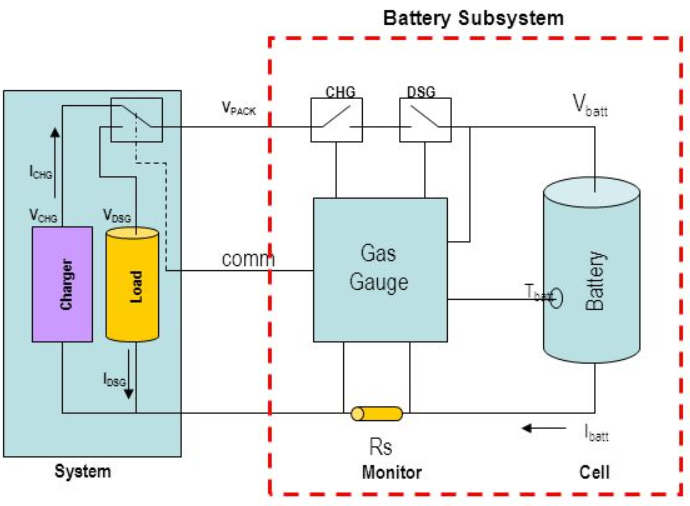
\includegraphics[width=12cm]{billeder/battery_management_block.png}
	\caption{Blokdiagram over batteristyresystem}
	\label{fig:battery_management_block}
\end{figure}

De primære formål med en BMS er som følgende:
\begin{itemize}[noitemsep]
	\item Minimere risikoen for beskadigelse af celler
	\item Overvåge og kontrollere en batteripakkes op- og afladningsprocess
	\item Estimere kapacitet
	\item Logge information
\end{itemize}


\section{Cellebalancering}
Ideelt set er alle battericeller produceret ens med samme egenskaber og opfører sig ens under hele cellens leve tid. Desværre er det langt fra virkeligheden, hvor der er produktionstolerancer, hvor nogle celler vil være stærkere end andre. I praksis betyder det varians på minimal, nominal og maksimal spænding, kapacitet, indre modstand og selvafladning.
Temperaturforskelle i en batteripakke og dermed forskelle på celletemperature kan også medføre varians på selvafladning over tid.
\\

\begin{figure}[h]
	\centering
	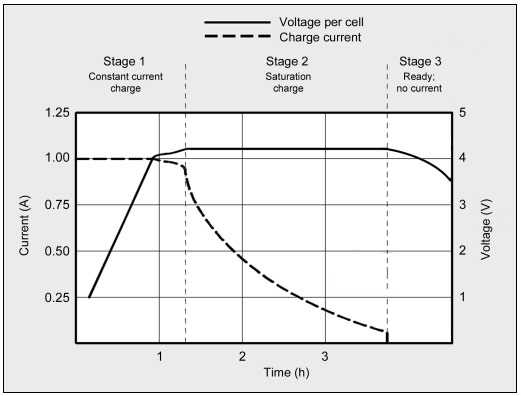
\includegraphics[width=15cm]{billeder/liion_opladning.png}
	\caption{Oplade forløb af Lithium-Ion celle}
	\label{fig:opladning_liion}
\end{figure}
\FloatBlock

I batteripakker hvor flere celler indgår, vil forskelle på stærke og svage celler forstørres for hver cyklus. Under opladning kan en svag celle blive svagere indtil den fejler, hvilket kan forsage permanent skade på hele batteripakken. Da en batteripakkes levetid afhænger af den svageste celle, vil en forøgelse i levetid kunne opnås ved hjælp af cellebalancering, da slid på den svageste celle minimeres. Opladning af en Li-Ion celle foregår i tre faser og er skitseret på figur \ref{fig:opladning_liion}.
\klp{Fase 4 skal fjernes da vi ikke har det med}
Under den første fase oplades cellerne med en konstant strøm, hvor spændingen stiger lineært. Det er i denne fase hvor størstedelen af
\\

I anden fase påbegyndes når den første celle er fuldt opladet, hvilket kan ses ved at cellespændingen når $V_{EOC}$ (End Of Charge) som typisk ligger på $V_{EOC} = 4.2 \volt$. Herefter påbegyndes balancering af cellerne, hvor den opladte celle aflades for efterfølgende at blive opladt sammen med de andre celler indtil de alle antager samme spænding.
Fasen kan siges at være opladning ved konstant spænding (der er en dog rippel spænding grundet balancering).
\\

Tredje og sidste fase er når cellerne har færdiggjort sin ladecyklus og går på standby. Grundet cellernes indre modstand, vil de langsomt aflades, hvilket ses på den nedadgående spændingsflanke.

\subsection{Passiv balancering}
Blanceringsteknikkerne kan opdeles i to kategorier: passiv og aktiv balancering.
\\
Passiv balancering går ud på at de omdanne overskudsenergi til varme fra fuldt opladte celler, modsat aktiv balancering som flytter overskudenergien til lavere opladte celler.
\\

Under passiv balancering holder systemet øje med spændingen på de enkelte celler. Når en eller flere celler opnår maks cellespænding $V_{EOC}$ og derved er fuldt opladet, aflades de igennem en modstand til de har samme spænding som den laveste celle i systemet eller en spændingsreference. Efterfølgende oplades alle celler igen, og denne proces vil forsætte indtil alle celler er fuldt opladet. Afladningsmetoden hedder controlled shunting resistor og er vist på figur \ref{fig:passiv_balancering_teknik}. 


%Denne metode har MOSFET i parallel med hver enkelt celle og kan styres simpelt ved hjælp af en comparator som får en MOSFET til at tænde for indkobling af en afladningsmodstand. Microcontrolleren vil samtidig overvåge samtlige cellespændinger, og vil derfor have styr på om hvorvidt der er behov for balancering.

Fordelen ved denne metode er at den er simpel og pålidelig, men tilgengæld er den ineffektiv, da al overskudsenergi omdannes til varme og dermed er spildt.

\begin{figure}[h]
	\centering
	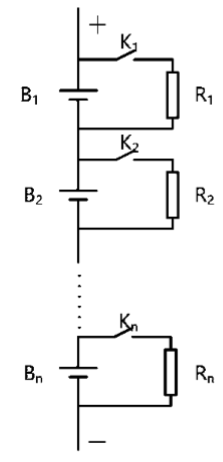
\includegraphics[width=10cm]{billeder/passiv_balancering.png}
	\caption{Passiv balancering gennem en færdig BMS chip.}
	\label{fig:passiv_balancering_teknik}
\end{figure}
\klp{Billede og tekst skal fikses. Balancering på IC er 70mA intern, så det bliver kravet. Med IC er ekstern balancerings FET ikke nødvendig. Vi matcher den diskret opbyggede til 50mA. Muligvis nyt billede da der er en modstand for meget.}




\subsection{Aktiv balancering}
Fælles for de aktive balanceringsteknikker er at de redistribuerer energi fra celler med høj ladning til celler med lav. På den måde mindskes tabet i forhold til passiv balancering hvor overskuds energi er ren tab. Da der i visse applikationer kan forekomme mange celler kan der være langt fra en celle der skal afgive energi til en der skal modtage, hvilket vil medføre et energi tab i transport.

Aktiv balancering kan opdeles i XXX topologier:

Fordele og ulemper
\\

Charge shuttles
\\

Aktiv balancering tillader større balanceringsstrømme end passiv balancering, meget af energien bliver redistribueret i stedet for omdannet til varme. 





\section{Estimering af kapacitet}
\klp{Mangler at få styr på denne sektion}
En af de vigtigste funktionaliteter i et batteristyresystem er estimering af kapacitet, State of Charge (SoC), og er direkte defineret som den procentdel af maksimal ladning i en celle eller en batteripakke. SoC er vigtig da det afspejler batteripakkens ydeevne. Nøjagtig estimering af SoC er ikke kun vigtig til beskyttelse af cellerne, men også for at forhindre overopladning og underafladning, hvilket bidrager til forlængelse af batteripakkens levetid. Dertil muliggør informationen også at lade batteristyresystemet ligge rationelle strategier for at spare energi.
\\
Informationen kan også bruges til at indikere behov tilslutning af oplader til brugeren gennem f.eks. en statusindikator eller om afladning af systemet kan tillades. 
Ved strømsvigt hvor f.eks et UPS-anlæg (Uninterruptible power supply) skal levere nødstrøm indtil normal drift genoprettes, vil SoC bidrage med information om hvorvidt anlægget overhovedet vil være i stand til at understøtte den tilkoblede belastning.
\\

SoC i en celle defineres som forholdet mellem nuværende ladning $Q_{t}$ og $Q_{n}$, hvilket er den nominelle ladning og er givet fra producenten, og er den maksimale ladning der kan opbevares i en celle.

\begin {equation} 
SoC(t) = \frac{Q_t}{Q_n} \label{eq:soc}
\end {equation}

Der anvendes typisk tre metoder til at afgøre SoC, gennem en direkte måling af cellespænding, ved at tælle ladning, og en blanding af disse to.

\subsection{Måling af terminalspænding}
Ved denne metode vil en simpel spændingsmåling henover cellerne kunne indikere kapaciteten, da spændingen på en celle tilnærmelsesvis falder lineært under afladning i dette projekts valgte arbejdsområde. Den er dog ikke så præcis, da det reelle afladningskurve ikke er lineær.


\subsection{Coulomb-tælle metode}
Denne metode går ud på at måle afladningsstrømmen i en batteripakke og integrere strømmen over tid, for at estimere realtids-kapaciteten $SoC(t)$. 

\begin {equation} 
SoC(t) = SoC(0) - \frac{1}{C} \int_{0}^{t} idt  \label{eq:coulomb-count}
\end {equation}

Overstående ligning kan forenkles,

\begin {equation} 
SoC(t) = SoC(0) - \frac{1}{C} \int_{0}^{t} idt  \label{eq:coulomb-count}
\end {equation}

Disse to teknikker kan også kombineres for at give et mere nøjagtigt estimat af batteripakkens kapacitet.

\section{State of Health (SoH)}
Formålet med SoH er at give en indikation af hvilken ydeevne der kan forventes af en celle eller batteripakke i den nuværende tilstand, eller fortælle noget omkring den resterende levetid før der er behov for udskiftning.
\\
I nogle applikationer bliver SoH løbende gemt i en logbog for validere

\begin {equation} 
SoH = \frac{nominel \space kapacitet - nuværende  kapacitet}{nominel kapacitet} \label{eq:soh}
\end {equation}
%    05609223.pdf

\begin {equation} 
SOH(t) = SOH(0) - \frac{1}{2N*E_{0}(0)}d \int_{0}^{t} P_{i}(t)dt
\end {equation}




\section{Temperaturmåling}
Måling af temperature i en batteripakke er nødvendig, for at sikre optimal op- og afladningsforhold. Alt afhængig vigtigheden af kendskab til temperaturene forskellige steder, kan der være flere temperaturmålere. Placeringerne er typisk på PCB'et og cellerne.
\\

Temperaturmålingen kan blive brugt flere steder i en batteripakke. Værdien kan indgå som en parameter til udregning af cellernes helbredsmæssige tilstand og til at sikre, at cellerne ikke blive op- og afladt under for kølige eller varme temperaturer. Når temperaturen næsten er for høj eller for lav, kan en batteripakke designes således at den kun tillader en begrænset indadgående eller udadgående strøm.

\section{Op- og afladningskontrol samt kortslutningsbeskyttelse}
For at isolere batteripakken fra belastning og oplader i tilfælde af fejl ved op- og afladning, skal BMS'en kunne afbryde forbindelsen mellem opladeren eller belastningen. Det kan realiseres ved hjælp af en oplade og aflade MOSFET som sammen virker som en to vejs kontakt kontakt i fejlsituationer, også kaldet cutott-MOSFETs. Opførelsen af cutoff-MOSFEN'en er typisk defineret ud fra parametre som maksimums værdier af cellespændinger, strømtræk og temperatur. 
\
